\documentclass[10pt]{article}
\usepackage{graphicx}

\begin{document}
\title{CSE616 Neural Networks and Their Applications\\
Assignment 1 Submission}
\author{Ayman Wagih Mohsen (2000728)}
\maketitle

\section{Question 1}

Layer 1 weights:
\[
	W_{L1}=
	\left[
	{
		\begin{array}{ccc}
		2&1&3\\
		2&-1&1\\
		\end{array}
	}
	\right],\quad
	b_{L1}=
	\left[
	{
		\begin{array}{c}
		1\\
		0\\
		-1\\
		\end{array}
	}
	\right]
\]
Layer 2 weights:
\[
	W_{L2}=
	\left[
	{
		\begin{array}{c}
		3\\
		1\\
		2\\
		\end{array}
	}
	\right],\quad
	b_{L2}=1
\]
Data sample:
\[
	x=
	\left[
	{
		\begin{array}{c}
		1\\
		3\\
		\end{array}
	}
	\right],\quad
	y=32
\]

1.a. Linear acitvation functions:\\
Layer 1 output:
\[
	net_{a}=W_{L1}^T x + b_{L1}=
	\left[
	{
		\begin{array}{cc}
		2&2\\
		1&-1\\
		3&1\\
		\end{array}
	}
	\right]
	\left[
	{
		\begin{array}{c}
		1\\
		3\\
		\end{array}
	}
	\right]+
	\left[
	{
		\begin{array}{c}
		1\\
		0\\
		-1\\
		\end{array}
	}
	\right]=
	\left[
	{
		\begin{array}{c}
		9\\
		-2\\
		5\\
		\end{array}
	}
	\right]
\]

Layer 2 output:
\[
	net_{\hat{y}}=W_{L2}^T a + b_{L2}=
	\left[
	{
		\begin{array}{ccc}
		3&1&2\\
		\end{array}
	}
	\right]
	\left[
	{
		\begin{array}{c}
		9\\
		-2\\
		5\\
		\end{array}
	}
	\right]+1=36
\]
The output $\hat{y}$ is 36.

1.b. ReLU activations:\\
Layer 1 output:
\[
	a=ReLU(net_{a})=
	\left[
	{
		\begin{array}{c}
		9\\
		0\\
		5\\
		\end{array}
	}
	\right]
\]

Layer 2 output:
\[
	net_{\hat{y}}=W_{L2}^T a + b_{L2}=
	\left[
	{
		\begin{array}{ccc}
		3&1&2\\
		\end{array}
	}
	\right]
	\left[
	{
		\begin{array}{c}
		9\\
		0\\
		5\\
		\end{array}
	}
	\right]+1=38
\]
\[
	\hat{y}=ReLU(net_{\hat{y}})=38
\]

1.c. Partial derivatives with linear activations:\\
The loss function:
\[J=(\hat{y}-y)^2\]
Partial derivative w.r.t layer 2 bias $b_1^{[2]}$:
\[
	\frac{\partial J}{\partial b_1^{[2]}}=
	2(\hat{y}-y)\frac{\partial \hat{y}}{\partial b_1^{[2]}}
\]
\[
	\hat{y}=w_{11}^{[2]}a_1+w_{21}^{[2]}a_2+w_{31}^{[2]}a_3+b_1^{[2]}
\]
\[
	\frac{\partial \hat{y}}{\partial b_1^{[2]}}=1
\]
\[
	\frac{\partial J}{\partial b_1^{[2]}}=
	2(\hat{y}-y)=2(36-32)=8
\]

Partial derivative w.r.t layer 2 weight $w_{21}^{[2]}$ from middle node $a_2$:
\[
	\frac{\partial J}{\partial w_{21}^{[2]}}=
	2(\hat{y}-y)\frac{\partial \hat{y}}{\partial w_{21}^{[2]}}
\]
\[
	\hat{y}=w_{11}^{[2]}a_1+w_{21}^{[2]}a_2+w_{31}^{[2]}a_3+b_1^{[2]}
\]
\[
	\frac{\partial \hat{y}}{\partial w_{21}^{[2]}}=a_2
\]
\[
	\frac{\partial J}{\partial w_{21}^{[2]}}=
	2(\hat{y}-y)a2=2(36-32)\times(-2)=-16
\]

Partial derivative w.r.t layer 1 bias $b_2^{[1]}$ from middle node $a_2$:
\[
	\frac{\partial J}{\partial b_{2}^{[1]}}=
	2(\hat{y}-y)\frac{\partial \hat{y}}{\partial b_2^{[1]}}
\]
\[
	\hat{y}=w_{11}^{[2]}a_1+w_{21}^{[2]}a_2+w_{31}^{[2]}a_3+b_1^{[2]}
\]
\[
	a_2=w_{12}^{[1]}x_1+w_{22}^{[1]}x_2+b_2^{[1]}
\]
\[
	\frac{\partial a_2}{\partial b_2^{[1]}}=1
\]
\[
	\frac{\partial \hat{y}}{\partial b_2^{[1]}}=w_{21}^{[2]}
\]
\[
	\frac{\partial J}{\partial b_2^{[1]}}=
	2(\hat{y}-y)w_{21}^{[2]}=2(36-32) \times 1=8
\]

Partial derivative w.r.t layer 1 weight $w_13^{[1]}$ from last node $a_3$:
\[
	\frac{\partial J}{\partial w_{13}^{[1]}}=
	2(\hat{y}-y)\frac{\partial \hat{y}}{\partial w_13^{[1]}}
\]
\[
	\hat{y}=w_{11}^{[2]}a_1+w_{21}^{[2]}a_2+w_{31}^{[2]}a_3+b_1^{[2]}
\]
\[
	a_3=w_{13}^{[1]}x_1+w_{23}^{[1]}x_2+b_3^{[1]}
\]
\[
	\frac{\partial a_3}{\partial w_{13}^{[1]}}=x_1
\]
\[
	\frac{\partial \hat{y}}{\partial w_{13}^{[1]}}=w_{31}^{[2]}x_1
\]
\[
	\frac{\partial J}{\partial w_{13}^{[1]}}=
	2(\hat{y}-y)w_{31}^{[2]}x_1=2(36-32) \times 2 \times 1=16
\]

1.d. One step of gradient descent (learning rate $\eta=2$):
\[
	new b_2^{[1]}=b_2^{[1]}-\eta\frac{\partial J}{\partial b_2^{[1]}}=0-2 \times 8=-16
\]
\[
	new w_{13}^{[1]}=w_{13}^{[1]}-\eta\frac{\partial J}{\partial b_2^{[1]}}=3 - 2 \times 16=-29
\]

1.e. In this problem, the model with identity activation produces results closer to the ground truth than the model with ReLU activation. But given that we have only one data sample, it is not enough data to judge which model will perform better in general. Also, the data samples should be divided into training and testing sets.


\newpage
\section{Question 2}
Function definitions:
\[
	g_1(x_1, x_2)=x_1 exp(x_2),\quad g_2(x_1, x_2)=x_1+x_2^2
\]
\[
	f(g_1, g_2)=sin(g_1)+g_2^2
\]
Partial derivatives by chain rule:
\[
	\frac{\partial f}{\partial x_1}=
	\frac{\partial f}{\partial g_1}\times\frac{\partial g_1}{\partial x_1}+
	\frac{\partial f}{\partial g_2}\times\frac{\partial g_2}{\partial x_1}
\]
\[
	\frac{\partial f}{\partial x_2}=
	\frac{\partial f}{\partial g_1}\times\frac{\partial g_1}{\partial x_2}+
	\frac{\partial f}{\partial g_2}\times\frac{\partial g_2}{\partial x_2}
\]
\[
	\frac{\partial f}{\partial g_1}=cos(g_1),\quad
	\frac{\partial f}{\partial g_2}=2g_2
\]
\[
	\frac{\partial g_1}{\partial x_1}=exp(x_2),\quad
	\frac{\partial g_1}{\partial x_2}=x_1 exp(x_2)
\]
\[
	\frac{\partial g_2}{\partial x_1}=1,\quad
	\frac{\partial g_2}{\partial x_2}=2x_2
\]
Substitute:
\[
	\frac{\partial f}{\partial x_1}=cos(g_1)exp(x_2)+2g_2 \times 1
\]
\[
	\frac{\partial f}{\partial x_2}=cos(g_1) x_1 exp(x_2)+2g_2 \times 2x_2
\]


\newpage
\section{Question 3}
3.1. Derivative of
\[f(z)=1/(1+exp(-z))\]
Solution:
\[
	f'(z)=\frac{-1}{(1+exp(-z))^2}exp(-z)\times (-1)
	=\frac{exp(-z)}{(1+exp(-z))^2}
\]
\[
	f'(z)=\frac{1}{1+exp(-z)}\frac{exp(-z)}{1+exp(-z)}
	=\frac{1}{1+exp(-z)}\left(1-\frac{1}{1+exp(-z)}\right)
\]
\[
	f'(z)=f(z)(1-f(z))
\]

3.2. Gradient of:
\[
	f(w)=\frac{1}{(1+exp(-w^T x))}
\]
Solution:
\[
	\frac{d f(w)}{d w_i}=
	\frac{d f(w)}{d net}\times x_i=
	f(w)(1-f(w))x_i
\]
\[
	\nabla f(w)=f(w)(1-f(w))\textbf{x}
\]

3.3. Derivative of:
\[
	J(w)=\frac{1}{2}\sum_{i=1}^m\left|w^T x^{(i)}-y^{(i)}\right|
\]
Solution (assuming data pairs $(x^{(i)}, y^{(i)})$):
\[
	\frac{\partial J}{\partial w}=
	\frac{1}{2}\sum_{i=1}^m sgn\left(w^T x^{(i)}-y^{(i)}\right)x^{(i)}
\]

3.4. Derivative of:
\[
	J(w)=\frac{1}{2}\left(sum_i=1^m\left(w^T x^{(i)}-y^{(i)}\right)^2\right)+\lambda\left||w\right||_2^2
\]
Solution:
\[
	J(w)=\frac{1}{2}\left(sum_i=1^m\left(w^T x^{(i)}-y^{(i)}\right)^2\right)
	+\lambda\left(\sum_j=1^n w_j^2\right)
\]
\[
	\frac{\partial J}{\partial w}=
	\frac{1}{2}\left(\sum_{i=1}^m 2\left(w^T x^{(i)}-y^{(i)}\right)\textbf{x}^{(i)}\right)
	+2\lambda \textbf{w}
\]

3.5. Derivative of:
\[
	J(w)=\sum_{i=1}^m\left(
		y^{(i)}log(\sigma(w^T x^{(i)}))+(1-y^{(i)})log(1-\sigma(w^T x^{(i)}))
	\right)
\]
\[
	\frac{\partial J}{\partial w}=\sum_{i=1}^m\left(
		y^{(i)}\frac
			{\sigma(w^T x^{(i)})(1-\sigma(w^T x^{(i)}))}
			{\sigma(w^T x^{(i)})}
		+(1-y^{(i)})\frac
			{-\sigma(w^T x^{(i)})(1-\sigma(w^T x^{(i)}))}
			{1-\sigma(w^T x^{(i)})}
	\right)
\]
\[
	\frac{\partial J}{\partial w}=\sum_{i=1}^m\left(
		y^{(i)}(1-\sigma(w^T x^{(i)}))-(1-y^{(i)})\sigma(w^T x^{(i)})
	\right)
\]

3.6. Gradient of
\[
	f(w) = tanh(w^T x)
\]
Solution:
\[
	\nabla f(w)=\frac{1}{1-(w^T x)^2}\textbf{x}
\]


\newpage
\section{Programming}
The script neural\_net.py:

\begin{tiny}
\begin{verbatim}
import pandas as pd
import numpy as np

data=pd.read_csv('winequality-red.csv', sep=';').to_numpy()    #load data
np.random.shuffle(data)#random shuffle

totalsize=data.shape[0]
testsize=totalsize//2
print('%d samples: %d train, %d test'%(totalsize, totalsize-testsize, testsize))
test=data[:testsize, :]    #divide to train & test sets
train=data[testsize:, :]

'''
train-=train.mean(axis=0, keepdims=True)    #standardize
train/=train.std(axis=0, keepdims=True)
#print(train)
'''

def activation(x):
    return x*((x>0)*0.1+(x<0)*0.001)#leaky ReLU
def activation_derivative(x):
    return (x>0)*0.1+(x<0)*0.001#leaky ReLU

class NeuralNet:
    def __init__(self, nInputs, nHidden, nOutputs):
        #[12 inputs] FC 12x30 [30 hidden] FC 30 [1 output]
        self.nInputs=nInputs
        self.nHidden=nHidden
        self.nOutputs=nOutputs
        self.w1=np.random.normal(loc=0, scale=1, size=[self.nHidden, self.nInputs+1])
        self.w2=np.random.normal(loc=0, scale=1, size=[self.nOutputs, self.nHidden+1])
        self.x=np.zeros(shape=self.nInputs)
        self.net_h=np.zeros(shape=self.nHidden)
        self.h=np.zeros(shape=self.nHidden)
        self.net_yhat=np.zeros(shape=1)
        self.yhat=np.zeros(shape=1)
        self.y=np.zeros(shape=1)
        #print(self.w1.shape)
        #print(self.w2.shape)
    
    def forward(self, x, y)->np.float_:#eval data sample, returns error
        self.x=np.append(x, [1])
        self.y=y
        
        self.net_h=np.matmul(self.w1, self.x)
        
        self.net_h=np.append(self.net_h, [1])
        self.h=activation(self.net_h)
        
        self.net_y=np.matmul(self.w2, self.h)
        self.yhat=activation(self.net_y)
        
        return (self.yhat-y)**2
    
    def backward(self, rate):#update weights
        temp=rate*(self.yhat-self.y)*activation_derivative(self.net_y)
        self.w2-=temp*self.h
        
        sum=0
        for j in range(self.nHidden):
            sum+=self.w2[0][j]*activation_derivative(self.net_h[j])
        self.w1-=temp*sum*self.x


net=NeuralNet(11, 30, 1)
nIter=1000
learning_rate=0.0001
ndim=train.shape[1]
error_train0=0
error_train=0
np.seterr(all='raise')#convert RuntimeWarnings to errors
for it in range(nIter):
    try:
        error_train=0
        for sample in train:
            error=net.forward(sample[0:ndim-1], sample[ndim-1])
            error_train+=error
            net.backward(learning_rate)
        error_train/=train.shape[0]
        
        error_test=0
        for sample in test:
            error=net.forward(sample[0:ndim-1], sample[ndim-1])
            error_test+=error
        error_test/=test.shape[0]
        
        print('it %d: rate=%f, e_train=%f, e_test=%f'%(it, learning_rate, error_train, error_test))
    except:
        print('ERROR: it %d: rate=%f, e_train=%f'%(it, learning_rate, error_train))
        break
    if np.isnan(error_train) or np.isnan(error_test):
        break
    
    #if it!=0:
    #   learning_rate=(error_train0-error_train)**3
    error_train0=error_train

print('finish')
\end{verbatim}
\end{tiny}

Results:
The following figures show the training error with time at different learning rates. Figure \ref{fig:image1} shows the error values starting from iteration 0. Figure \ref{fig:image2} shows the error values starting from iteration 40.
\begin{figure}[p]
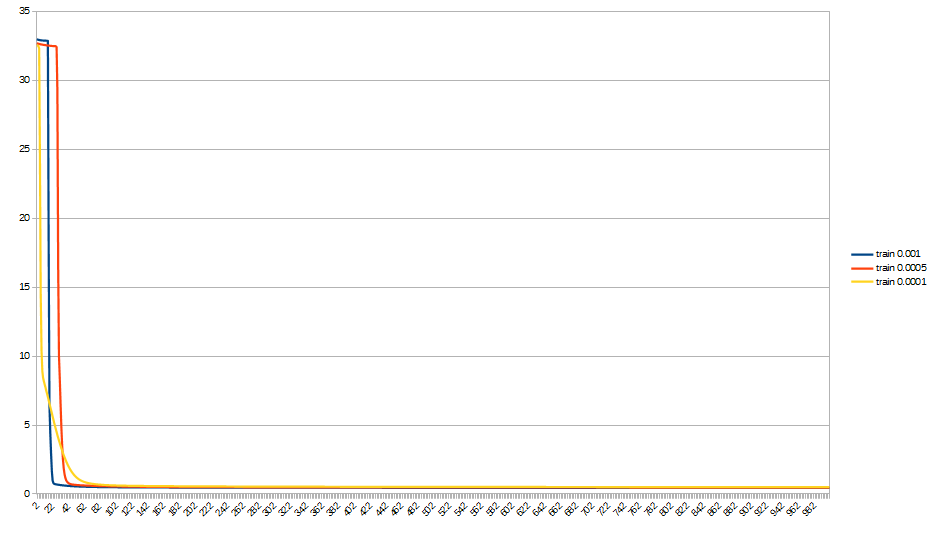
\includegraphics[width=0.9\textwidth]{20220409 4 results full.png}
\DeclareGraphicsExtensions{.png}
\caption[]{The error with time starting from iteration 0.}
\label{fig:image1}
\end{figure}
\begin{figure}[p]
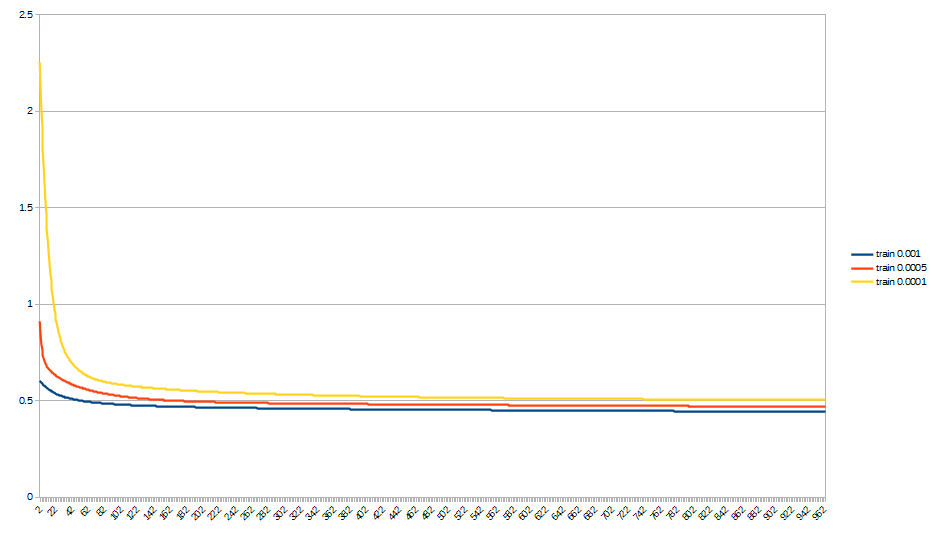
\includegraphics[width=0.9\textwidth]{20220409 4 results tail.png}
\DeclareGraphicsExtensions{.png}
\caption[]{The error with time starting from iteration 40.}
\label{fig:image2}
\end{figure}

\end{document}
